\chapter{Background / Related Work}

\section{Two-Dimensional Image Representation on Computers}
\label{sec:2dimages}

At it's most basic form, a sketch can be described as an image drawn on a planar two-dimensional surface.
With computer displays, there are two standard methods for generating two dimensional images: raster graphics and vector graphics.
The underlying data structures  have a large impact on the types of tools that can be designed to create, modify, and display the resulting images.

\subsection{Raster Graphics}

Raster graphics is an image format that uses a two-dimensional grid to represent each pixel in the image. 
A raster image is characterized by its width and height in pixels and by its color depth, the number of bytes per pixel. 
The depth value specifies the color for each pixel, usually by identifying the magnitude of the pixel's RGB components. 
The reasoning behind representing images by this method is that today most computer monitors have bitmapped displays. 
Today, although there are many standard formats, almost all displays consist of rectangular arrays of square pixels, and the bandwidth from the display's memory is sufficient enough to dynamically render multi-megapixel images. 
\begin{figure}
\fbox{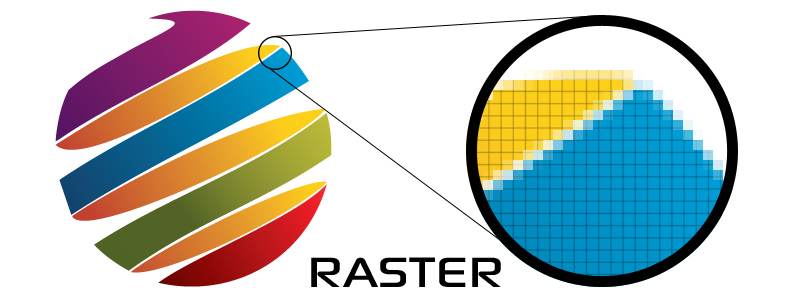
\includegraphics[width=\textwidth]{raster.jpg}}
\caption{Zooming in on a Raster Graphics Image \autocite{printingcollection}}
\end{figure}



When creating and editing raster graphics images, the software directly manipulates pixel values, also known as pixel editing.
This simplifies creating tools for editing raster graphics, since each tool can manually define how pixels are effected based on where and how an input occurs. 
Unfortunately, the ultimate quality of an image based on raster graphics is limited by the fact that the picture is resolution dependent. 
If you were to continuously zoom in on a raster image, eventually the image would suffer from image degradation. 
This resolution dependency also means that raster images are not flexible for working with extremely detailed environments.
It is possible for multiple small details to be contained inside of a single pixel.
Since a pixel can only store one color, all of these small details are lost.

\begin{figure}
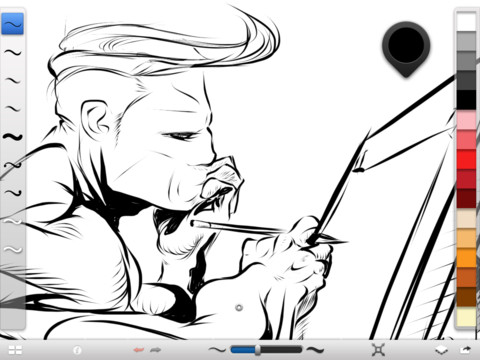
\includegraphics[width=\textwidth]{sketchbook.jpg}
\caption{Creating a Raster Image in Sketchbook}
\end{figure}



Examples of popular raster graphics software are Corel Painter\autocite{coreal}, Adobe Photoshop\autocite{photoshop}, Microsoft's MSPaint\autocite{mspaint}, the open-source GIMP software\autocite{gimp}, and Autodesk's Sketchbook\autocite{sketchbook}.

\subsection{Vector Graphics}

Vector graphics software uses geometrical primitives such as points, lines, curves, shapes and polygons to represent an image.
Each of these primitives has a defined geometric coordinate within the work space and determines the direction of the displayed vector. 
Vectors can also be assigned a variety of properties such as its color and thickness.
Although the resolution is limited by the computer's numerical precision, it is independent of the actual display. 

Because of their mathematical nature, they are theoretically similar to three-dimensional computer graphics, but the term specifically refers to two-dimensional images; in part to distinguish them from raster graphics.
Vector graphics are primarily used for line art, images drawn with distinct straight or curved lines.
For example, early CAD systems mostly used calligraphic black and white displays and rendered images in vector graphics formats. 
However, today, data in vector graphics form is now converted to raster graphics formats when used outside of vector specific editing software.  

Vector graphics data structures offer a number of advantages compared to raster approaches. 
First, they are based on mathematical expressions, which means they are resolution independent.
Zooming in on the image does not cause image degradation as in raster graphics; the image will remain smooth. 
Second, objects made using vector graphics are independent from their visual representation.
This allows for easy and accurate editing of primitives, provided they are contained in a vector graphics workspace.
For example, say we have an image of a circle covering a part of a square. In vector graphics, the circle can be moved without effecting the square beneath, because the data structure contains the information about both objects independently from their visual representation.
This type of editing is not possible in a single raster graphics image, because the underlying pixel representation does not contain the definition of objects in the image.
 

\begin{figure}
\fbox{
\includegraphics[width=\textwidth]{vector.jpg}}
\caption{Zooming in on a Vector Graphics Image \autocite{printingcollection}}
\end{figure}

\begin{figure}
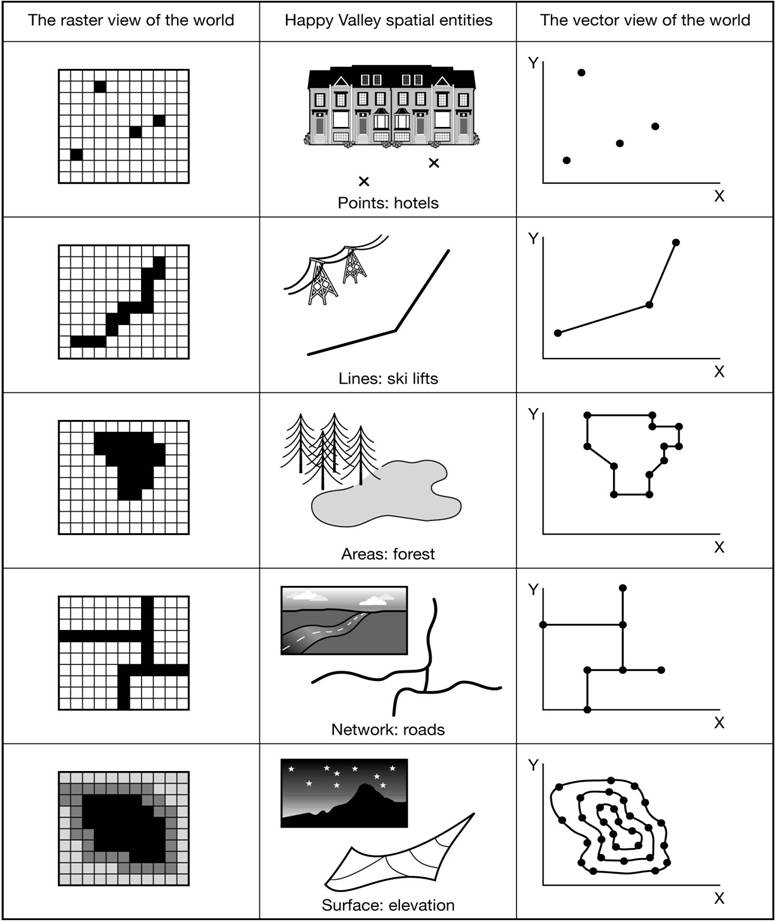
\includegraphics[width=\textwidth]{vector_raster.jpg}
\caption{Raster definition of an image vs Vector definition}
\end{figure}

Examples of popular vector graphics editing software are Adobe Illustrator\autocite{illustrator}, Corel Draw\autocite{coreldraw}, and Inkscape\autocite{inkscape}.

\subsection{Adaptive Distance Fields: Mischief}

Mischief\autocite{mischief} is a pseudo-vector graphics based drawing application. 
Although its underlying data structures are similar to those in other vector graphics applications, it does not allow for the precise editing of curves as seen in traditional vector graphics programs such as Adobe Illustrator. 
Instead it attempts to use vector graphics to simulate real world art techniques, similar to Sketchbook.
This is made possible by using a data-structure called Adaptive Distance Fields\autocite{asdf}, which stores vectors in a tree data structure instead of the traditional vector format.
Since the tree data structure ends up looking like a pseudo-raster, raster brushes and pens can be implemented in this system by defining what shapes go inside of the data structure.
Adaptive Distance Fields also greatly reduce the storage size of large scale vectors, making it possible for the implementation of their "infinite canvas"; their infinitely zoom-able, translatable workspace. 
This unique data structure allows for incredible detail and unlimited scale.

\begin{figure}
\centering
\fbox{\includegraphics[width=0.45\textwidth]{infinitecanvas1}}
\fbox{\includegraphics[width=0.45\textwidth]{infinitecanvas2}}
\caption{An example of the infinite canvas in Mischeif.}
\end{figure}

\section{3-D Sketching in CAD}

There have been many previous attempts to utilize 3-D sketching in the design process. In this section, we will describe some methods others have previously implemented either of published.

\subsection{CATIA Natural Sketch}

Natural Sketch is a feature inside of the CATIA modeling software\autocite{catia}. 
Natural Sketch allows the user to draw on a virtual plane, a 3-D model, and the plane where the screen lies in the 3D environment. 
It features the abilities to alter the pen style, alter the number of control points used to make the post sketch curve, automatically change the camera view to align with the drawing plane if one is being used, copy and alter individual strokes, and generate models from the 3-D sketch.

Natural Sketch uses a two-phase design system. 
First, the user creates a "rough sketch", where lines are rendered exactly as drawn. 
Afterwards, the user can trace over their already drawn lines to produce smooth curves from the initial sketch.
The traced curves are stored as Catmull-Clark splines.
While this system closely has the capabilities we would like to implement, it is currently only available in a solid modeling environment, making it incompatible with many tools most designers use to create early stage 3-D sketch models.

\begin{figure}
\centering     %%% not \center
\subfigure[Beginning the sketch ] {\label{fig:catia1}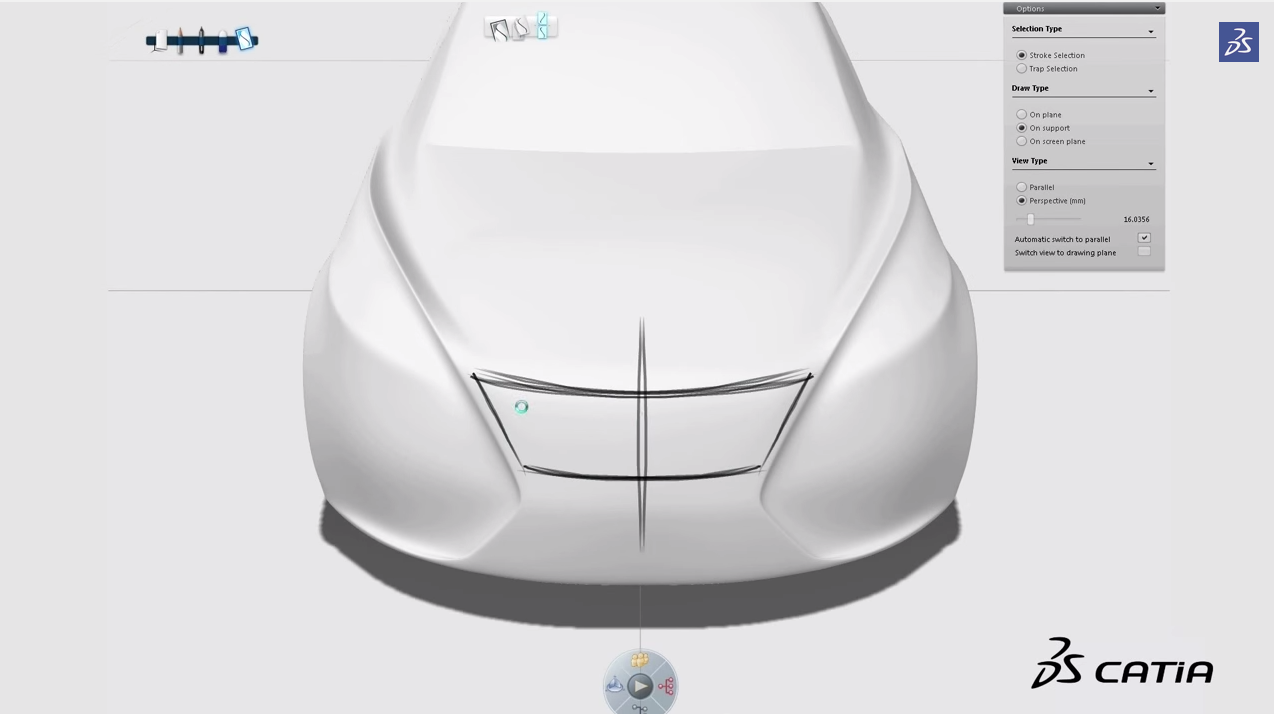
\includegraphics[width=\textwidth]{CATIA1}}
\subfigure[Finishing the sketch] {\label{fig:catia2}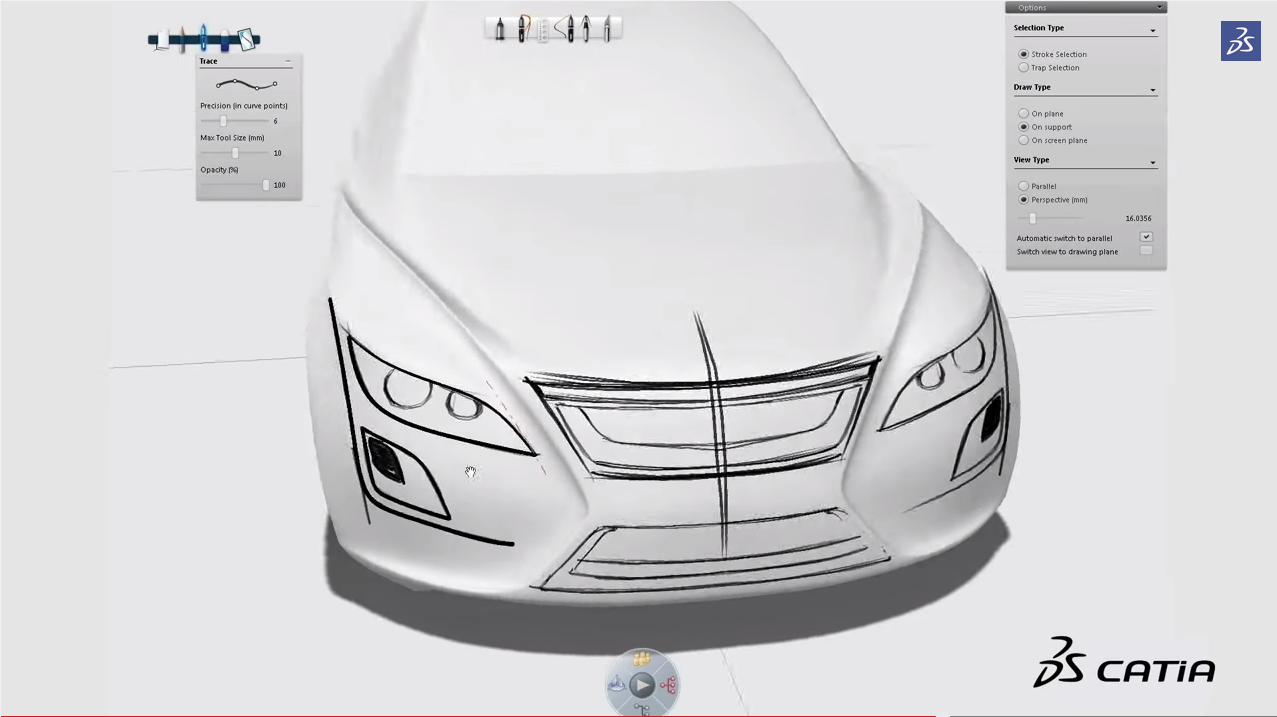
\includegraphics[width=\textwidth]{CATIA2}}
\caption{Using Natural Sketch to Add Detailing to a Car. \autocite{catiareel}}
\end{figure}

\subsection{EverybodyLovesSketch}

EverybodyLovesSketch\autocite{lovesketch} is a 3D curve sketching system from the University of Toronto's Dynamic Graphics Project Lab. It features a pen based gesture system, allowing the user to execute functions using rapid strokes, circles, and other predefined stroke patterns. Other features include dynamic sketch plane selection, single view definition of arbitrary extrusion vectors, multiple extruded surface sketching, copy-and-project of 3D curves, free-form surface sketching, and an interactive perspective grid. This project is based off of previous work by the same lab, ILoveSketch, which is the base 3D sketching functionality of the EverybodyLovesSketch project.

\subsection{Hyve3D}

\begin{figure}
\centering  
\subfigure[A user using an iPad to sketch on a plane inside of the virtual environment.] {\label{fig:hyve1}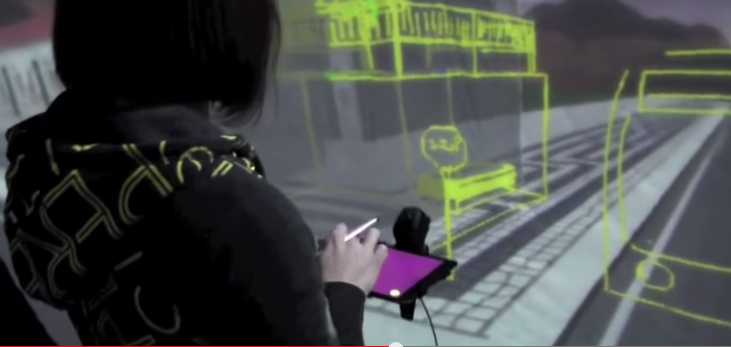
\includegraphics[width=\textwidth]{Hyve3D1}}
\subfigure[Manipulating the drawing plane by manipulating the iPad] {\label{fig:hyve2}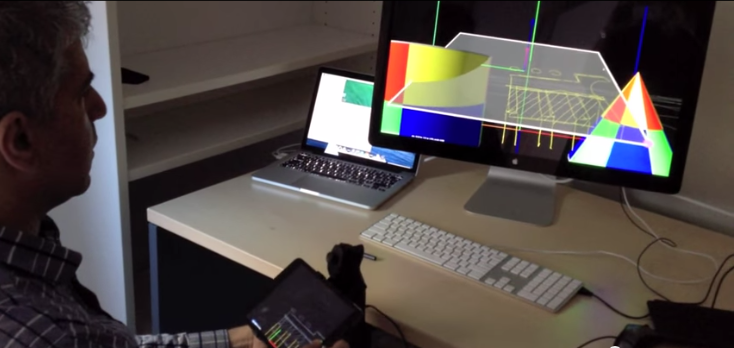
\includegraphics[width=\textwidth]{Hyve3D2}}
\caption{An example of using Hyve3D to draw inside of a virtual environment. \autocite{hyve3d}}

\end{figure}

Hyve3D\autocite{hyve3d} is an infinite virtual sketching environment from the University of Montreal. It uses two screens; a computer monitor to show the 3-D environment, and an iPad to draw. The sketching plane represented by the iPad is shown in the virtual environment, and is manipulated by moving and rotating the iPad in the real world. The user then pins the sketch plane in place and proceeds to draw at leisure. The advantage of this system is that it combines real world manipulation with virtual representation, eliminating the need for complex user interfaces and gestures. The disadvantage is that this kind of movement has no one-to-one feedback between the real world and the virtual, meaning that it is difficult to judge how your movements of the iPad effect the drawing place without confirming it visually.



\section{3-D Sketching in 3-D}

3-D content creation on a traditional computer screen is limiting. 
Any type of input or user interface can never overcome that one dimension of the workspace will always be inferred, due to the two dimensional output.
Work in this space explores alternative devices that work with methods of three
The result has been leveraging a number of emerging technologies that deal with output that is experienced in three dimensions. 


\subsection{Virtual Reality / Augmented Reality}

Recently, there have been two key technologies developed with the intention to immerse the user in a virtual environment; virtual and augmented reality. 
Both of these involve head-mounted displays (HMDs) that display two dimensional images.
Despite the images being flat, the system takes advantage of how humans see, such that the user feels the presence of actually being inside of the virtual environment.
The advantage to using these virtual systems is the user can use their sense of depth to fully understand the space they are working in.
The downside that these systems have is since their input methods are essentially drawing in midair, there is no tactile feedback similar to a pen pushing against a piece of paper.
An example of an augmented reality approach to 3-D sketching is Gravity Sketch, and one of a virtual reality approach is TiltBrush  by Skillman \& Hackett.

\begin{figure}
\includegraphics[width=\textwidth]{gravity1.png}
\includegraphics[width=\textwidth]{gravity2.png}
\caption{Augmented Reality Sketching using the Gravity tablet and Headset}
\end{figure}

\subsection{3-D Printing}

So far, we have only explored the idea that 3-D sketching is only possible in virtual environments, due to the inherent two dimensional techniques artists have used for centuries.  
However, groups have experimented with using 3-D printing to create pens that can sketch simple 3-D models; examples being the Polyes Q1 Pen and the 3Doodler.
These pens work similarly to hot glue guns, except instead of glue, the pens secrete ABS plastic that quickly hardens as it exits the tip of the pen.
Like the digital approaches, these pens lack tactile feedback, and rely purely on the user's sight to sketch.
Unfortunately, between the apparent structural instability of even small models created by the pen, as well as the lack of flexibility in the way the pen can be used, it appears that this route is impractical for creating the types of large and intricate structures seen in modern design, and is at best a toy.